\chapter{Device Orientation}
\label{Chapter:Orientation}
\begin{flushright} 
\textit{"If you do not change direction, you may end up where you are heading."\\
- Lao Tzu, Tao Te Ching}\end{flushright} 
\begingroup %\vspace*{\beforechapskip}% %\smash{\rule{2.6pt}{25mm}}
\textit{ On-body device orientation influences a variety of
 sensing modalities common in context recognition systems. 
 We discuss the effects orientation changes have on these modalities 
 and present a method to infer the orientation from the acceleration signal of a mobile device carried in a pocket. 
 Whereas previous work has shown how to determine the orientation in the vertical plane (angle
 towards earth gravity), we demonstrate how to compute the
 orientation within the horizontal plane. To validate our method we
 compare the results with GPS heading information when
 walking in a straight line. On a total of 16 different orientations
 and traces we get a mean difference of 5 degrees with 2.5 degrees
standard deviation.
}\\\\
Kai Kunze, Paul Lukowicz, Kurt Partridge, Bo Begole, Which Way Am I
Facing: Inferring Horizontal Device Orientation from an Accelerometer
Signal, \textit{13th IEEE International Symposium on Wearable
 Computers}. Linz, Austria, 2009.
\vskip\onelineskip
\begin{adjustwidth}{}{-\chapindent}%
\hrulefill
\end{adjustwidth}\endgroup
\vskip\onelineskip
\vskip\onelineskip 
\begin{figure}[t]
  \begin{center}
  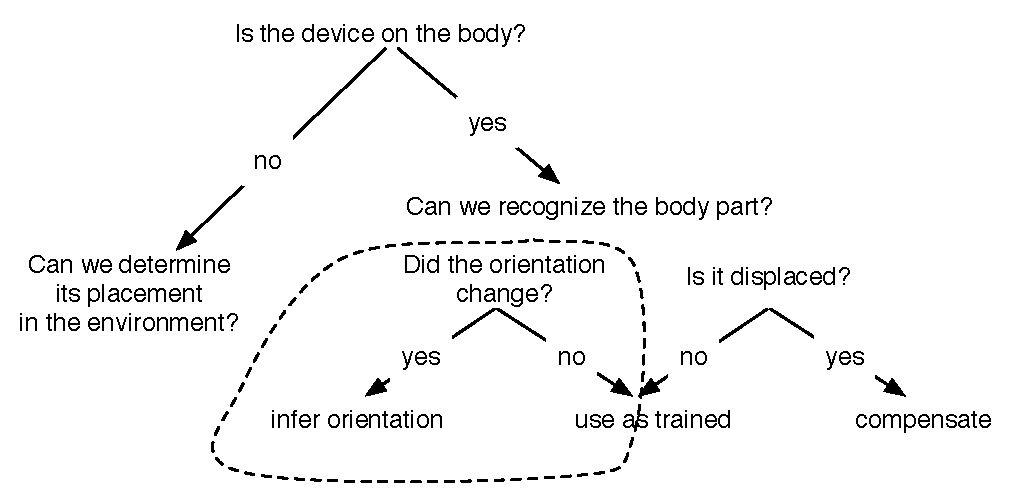
\includegraphics[height=2in]{orientation}
	\end{center}
\caption[Focus of the Orientation Chapter]{Thesis overview with the central question for this chapter
 highlighted.} \label{fig:orientationoverview} \end{figure}
The last type of finer grain placement variations we deal with is device orientation changes with respect to the user's body (see Figure~\ref{fig:orientationoverview}). 
When talking about orientation changes we mean changes of the reference system
of the sensor , e.g. turning a sensor 180 degrees around an arbitrary axis. The global position of the sensor stays unchanged.
For example, a mobile phone or other smart device can
be put into the pocket with the front facing towards or away from the
body. In addition, devices may rotate around the axis perpendicular to
the body, especially if they are small and lose in the pocket. Further, consider a mobile phone in a hip holster; usually, 
the device can be put into the holster in at least two ways:
display facing inwards or outwards. Sometimes there may also be the
option of attaching the holster either vertically or
horizontally. Finally, the holster can be placed at various locations
around the hip, which determines the exact horizontal orientation.
Similar considerations are possible with respect to the
placement inside the pocket. Especially in large trouser pockets, significant
variations in the orientation can occur when the device drifts from
one side of the pocket, e.g. on the front side of the leg, to the
other, e.g. on the side. 

For recognition systems using motion sensors, orientation information
can be important in two ways. First, it can improve recognition
performance by providing more detailed features (e.g. using all 3
individual axes of an accelerometer) than the orientation invariant
vector norm. Second, it can in itself be a relevant piece of
information. 
 
The next section shows how orientation changes influence common sensor
modalities. Afterwards, we detail related work to get a grasp on
already published approaches to the problem, followed by an
introduction and evaluation of our method to determine the on-body
device orientation in a trouser pocket based on acceleration signals from the smart device.


\section{Impact of Device Orientation}
\label{orient:impact}


\begin{figure}[t]
  \begin{center}
  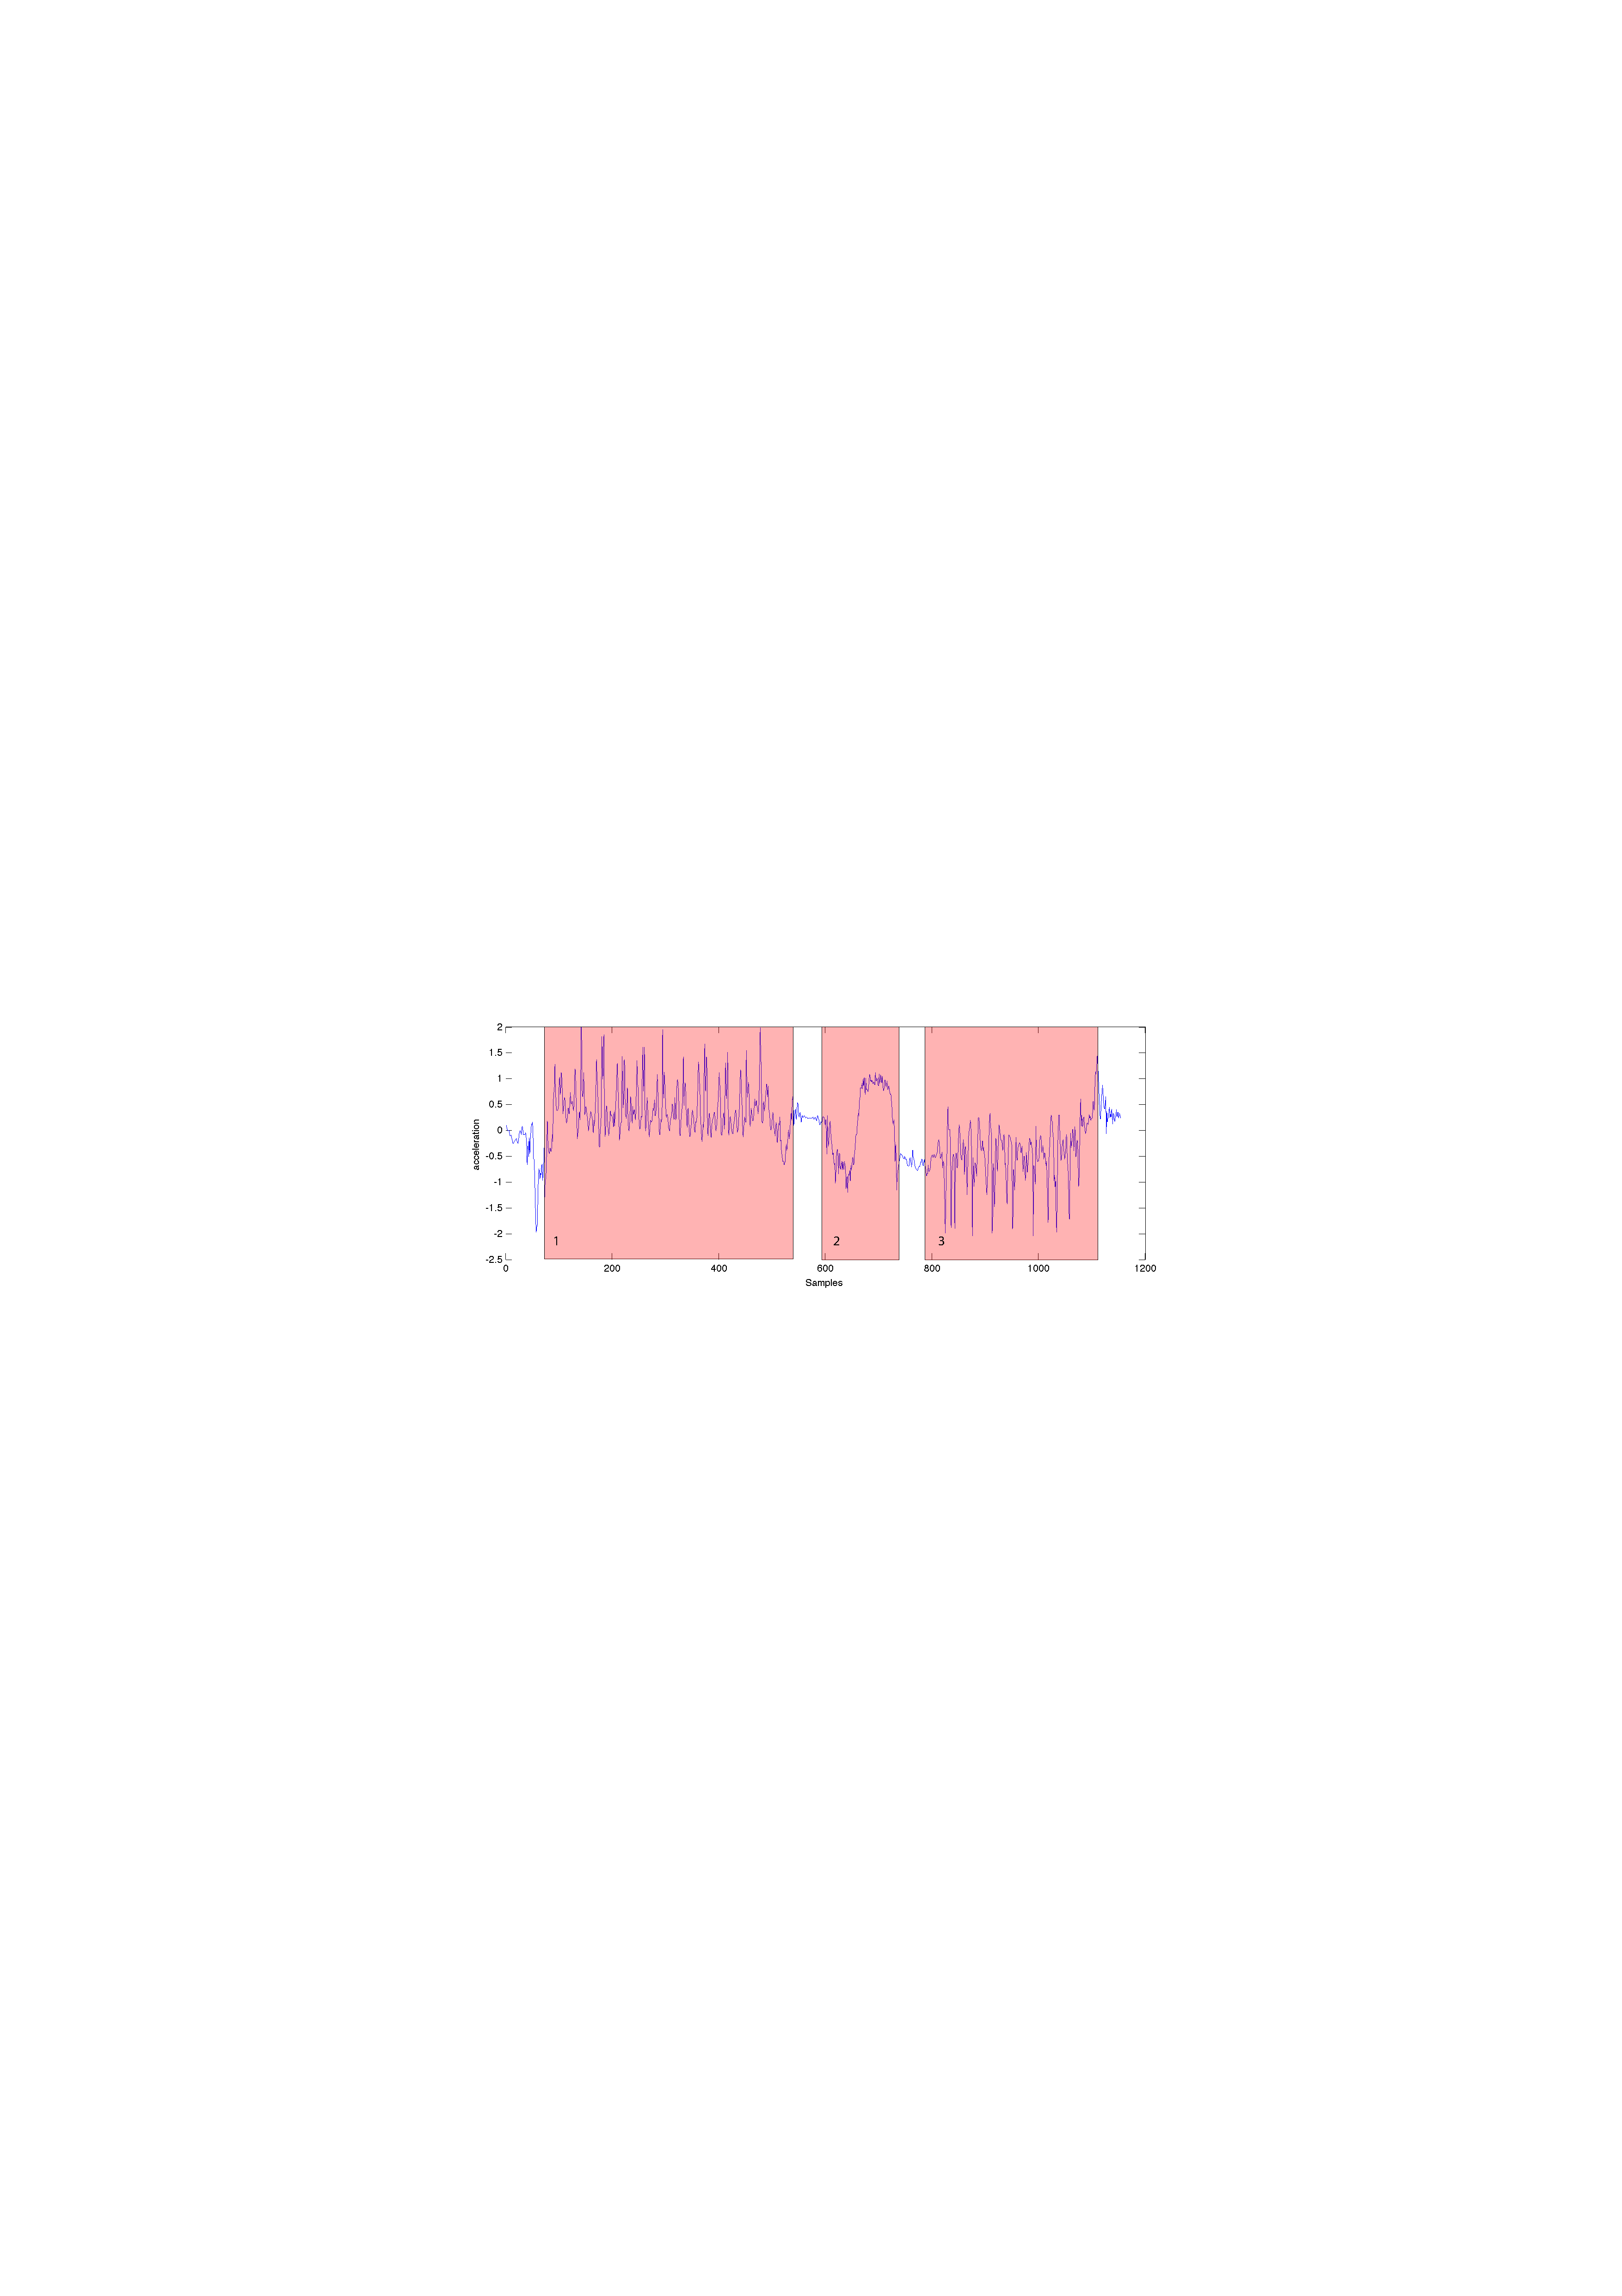
\includegraphics[height=2in]{acceleration-orientation}
	\end{center}
\caption[Orientation changes]{Effect of an device orientation change on one axis of an
 accelerometer with the user walking in phase 1, changing the
 orientation in 2, and walking again in
 3.} \label{fig:accelorient} \end{figure}

As to be expected motion sensors are highly affected by device
orientation changes relative to the user's body. 
The user's motion is distributed differently on the axes of the sensor depending on the
device orientation. For example, a user walks a bit, stops, takes out his mobile phone and 
places it back in the pocket turned by 180 degrees before continuing walking. 
The effects of this scenario on an accelerometer axis is illustrated in Figure~\ref{fig:accelorient}.
The user is walking with the device in the pocket during phase 1 indicated in the plot. 
The user takes out the device turns it 180 degrees (marked in phase 2), puts it back and continues walking in phase 3. 
With accelerometers not only the dynamic acceleration component (the user's motion) is distributed differently depending on
the orientation, but also the static gravity component shifts between axes. This is recognizable in Figure~\ref{fig:accelorient},
as the signal offset changes from 0.5 to -0.5 g from phase 1 to phase 3 (see the Displacement Chapter,
Section~\ref{dis:impacts} for more details).


\begin{figure}[t]
  \begin{center}
  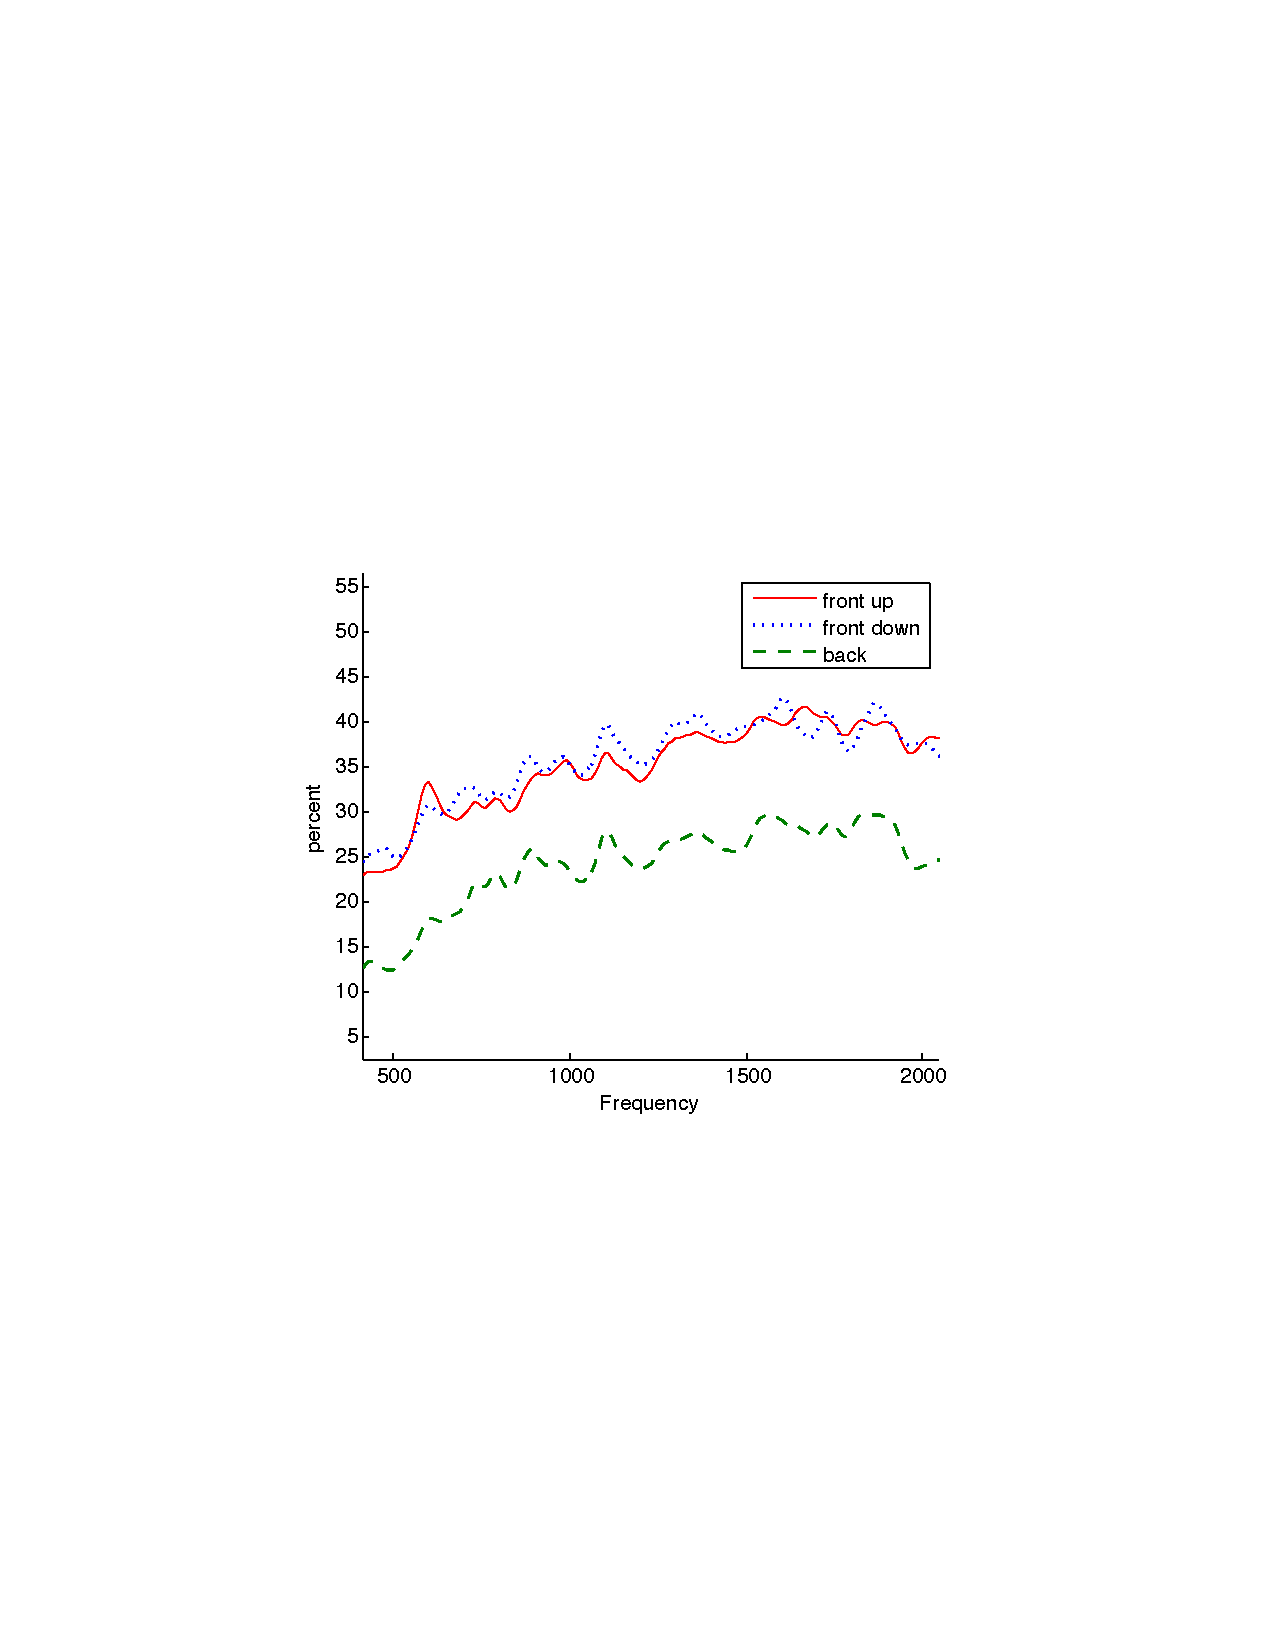
\includegraphics[height=2.0in]{iphoneAudio}
  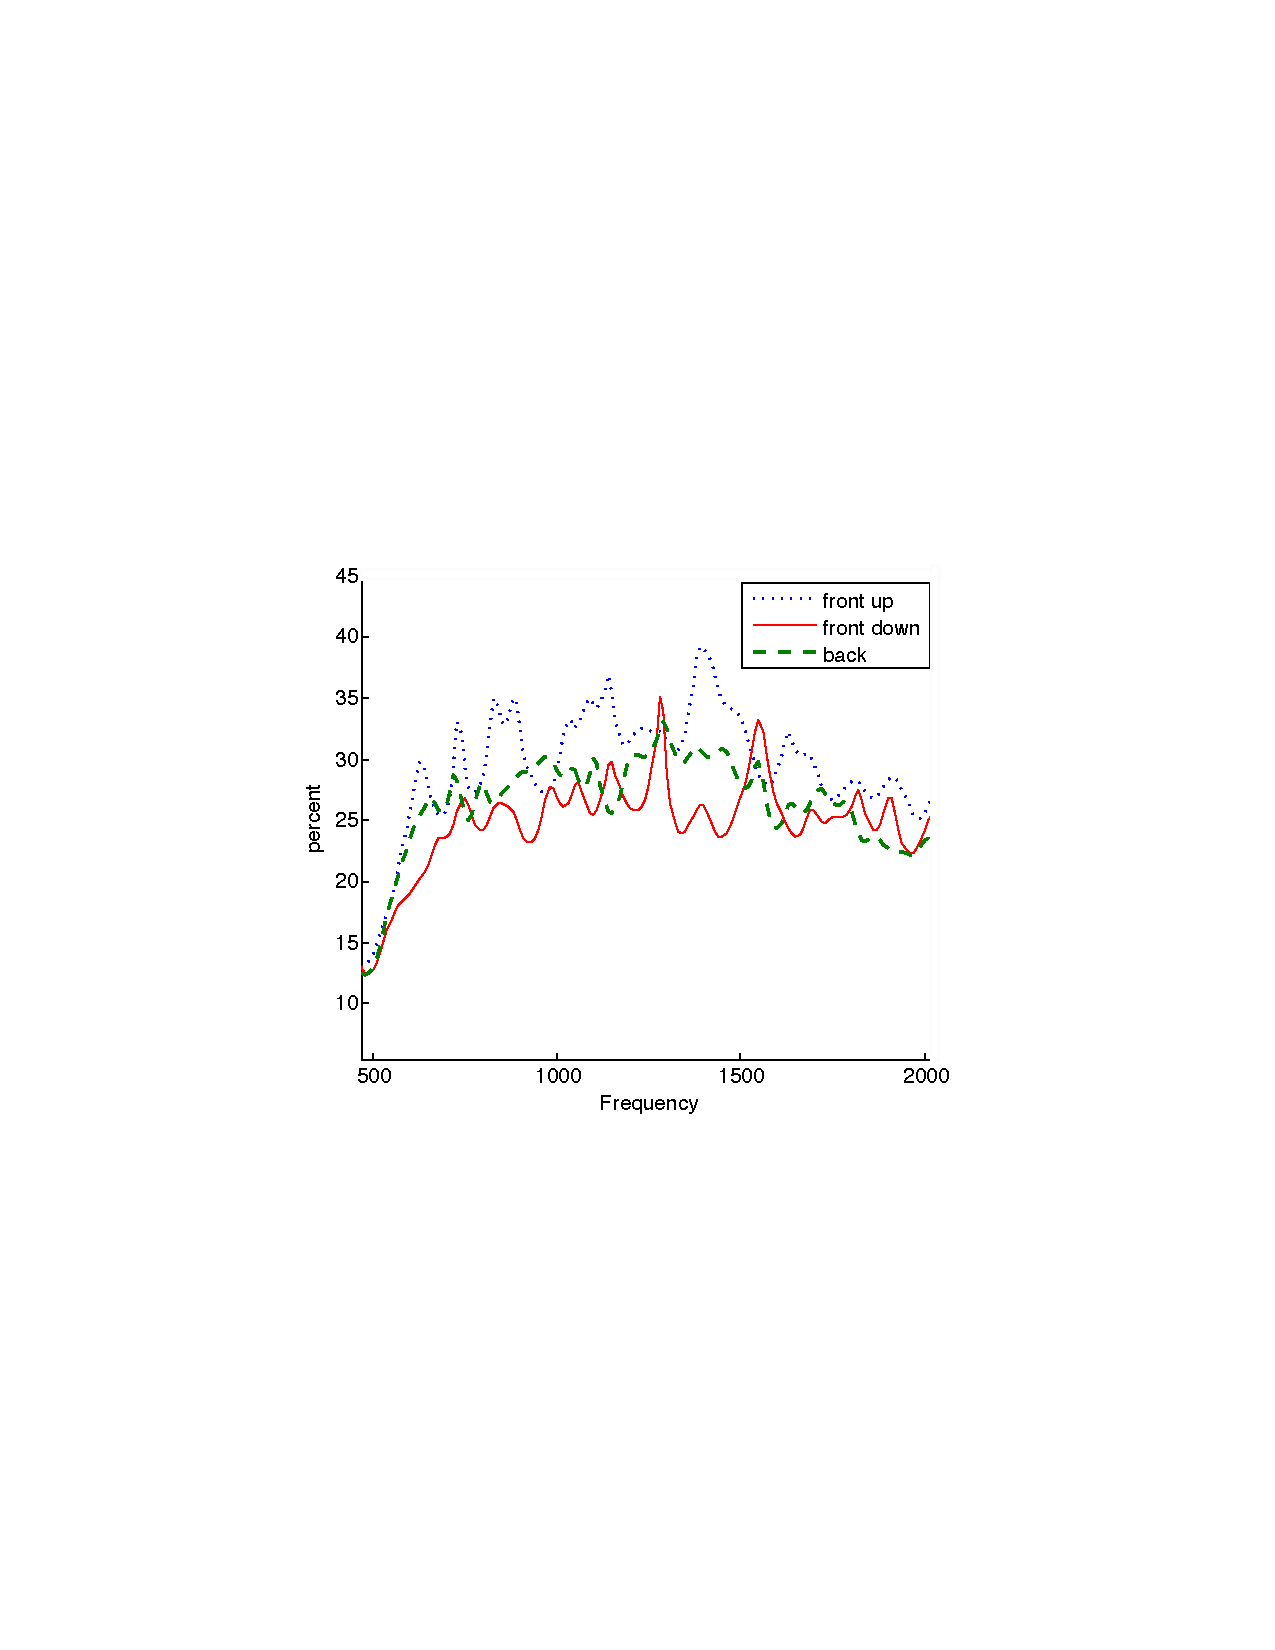
\includegraphics[height=2.0in]{nokiaAudio}
	\end{center}
\caption[Audio dampening due to device orientation]{Audio dampening depending on device orientation in a trousers pocket, in the left plot
 for the iphone and on the right for the nokia
 810i.} \label{fig:orientation_audio} \end{figure}

For sound, specific orientations can lead
to the microphone being directed towards the user rather than towards
the environment. This can significantly increase signal damping. Fix rules for the influence of orientation on signal damping are
difficult to formulate since the effect is strongly dependent on
device and clothing configuration. This is
illustrated in Figure~\ref{fig:orientation_audio} showing the influence of
the orientation on the audio signal absorption spectrum for the Nokia
810i and the iphone 3gs. We play white noise and record it with the respective device 
and changing device orientation in a trousers pocket. Figure~\ref{fig:orientation_audio} depicts the
frequency spectrum of the recorded audio. The Nokia 810i PDA
has its microphone on the front side. When in the trousers pocket
damping across all frequencies is larger if the device is facing
towards the body than when it's pointing away. As a counterexample
the same Figure~\ref{fig:orientation_audio} also shows the results of
this simple experiment done using the iphone, which has the microphones
on the lower side. Here orientation changes have only little effect.
Depending on where the microphone is located on the device, different orientation will
cause it to be more or less obstructed by the body or clothing.

\begin{figure}[t]
  \begin{center}
  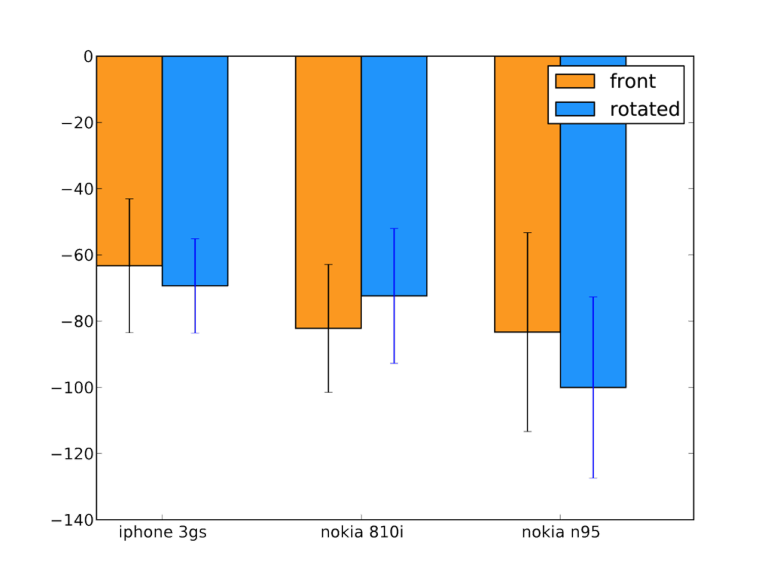
\includegraphics[height=2.0in]{orientWifi}
	\end{center}
\caption[Wifi signal strength variations]{The Figure shows the variation of WiFi signal strength
 measured for three different devices in different orientations.}
\label{fig:orientation_damping}
\end{figure}

For WiFi signal strength orientation effects depends highly on the position and properties of the antenna. 
To underline this we conduct a small test with three commodity handheld devices, the nokia 810i, n95 and
the iphone 3gs. We place them in the trousers pocket recording the
wlan signal strength for 10 min screen facing front and rotated by 180
degress (facing up side down). As seen in
Figure~\ref{fig:orientation_damping}, depending on the mobile the
orientation influences the signal strength differently.

Summing up, all given sensing modalities are affected by device
orientation relative to the user body in a non trivial way. Orientation effects
on sound and wifi depend highly on the given hardware and other environmental 
influences (e.g. the dampening of the clothes worn by the user). Therefore, we focus on motion sensors to estimate the
on-body orientation of a device.

\section{Related Work}
\label{sec:orient:related}

There is a significant push from research towards mobile phone sensing. 
Using mobile phones and other smart devices, device orientation becomes a major issue. Thus, there is quite some effort to make mobile phone inference more robust. 
Again, most researchers focus on orientation robust or indifferent features. 

Lester et al. presented a classification algorithm working accurately with data from different locations on the body~\cite{Lester:2006p31}. Pham and Abselzaher use features based on relative energy distribution to become more orientation independent~\cite{Pham:2008p146}. 

Another research effort centers around relative positioning and orientation between devices. For example, Pirkl et al. use magnetic resonance coils to calculate the orientation and distance between devices~\cite{pirkl}. This approach implies the use of two devices and gives only relative orientation and distance between them.

The closest to the work presented later in Section~\ref{sec:orientationdetection} is research from Henpraserttae et al.~\cite{Henpraserttae:2011fa}. They coin the orientation of the device as classification problem and uses the determined orientation to transform the reference coordinate system. As it is a classification problem the training complexity increases with the number of orientations, also the evaluation, so far, only uses four different orientations.

%From the related work above one can make out two distinct approaches
%towards dealing with device orientation. The first disregards
%recognition. The second tries to approximate the device orientation
%relative to the user's body, applies some transformation on the sensor
%signal and uses the transformed signals for inference. 

As seen, there are two approaches to deal with orientation changes in motion based context recognition:
\begin{enumerate}
\item to use aggregate features that are more robust or independent to orientation.
\item to try to infer the sensor orientation relative to the users body.
\end{enumerate}


\section{Loss of Orientation Information}



\begin{figure}[t]
  \begin{center}
  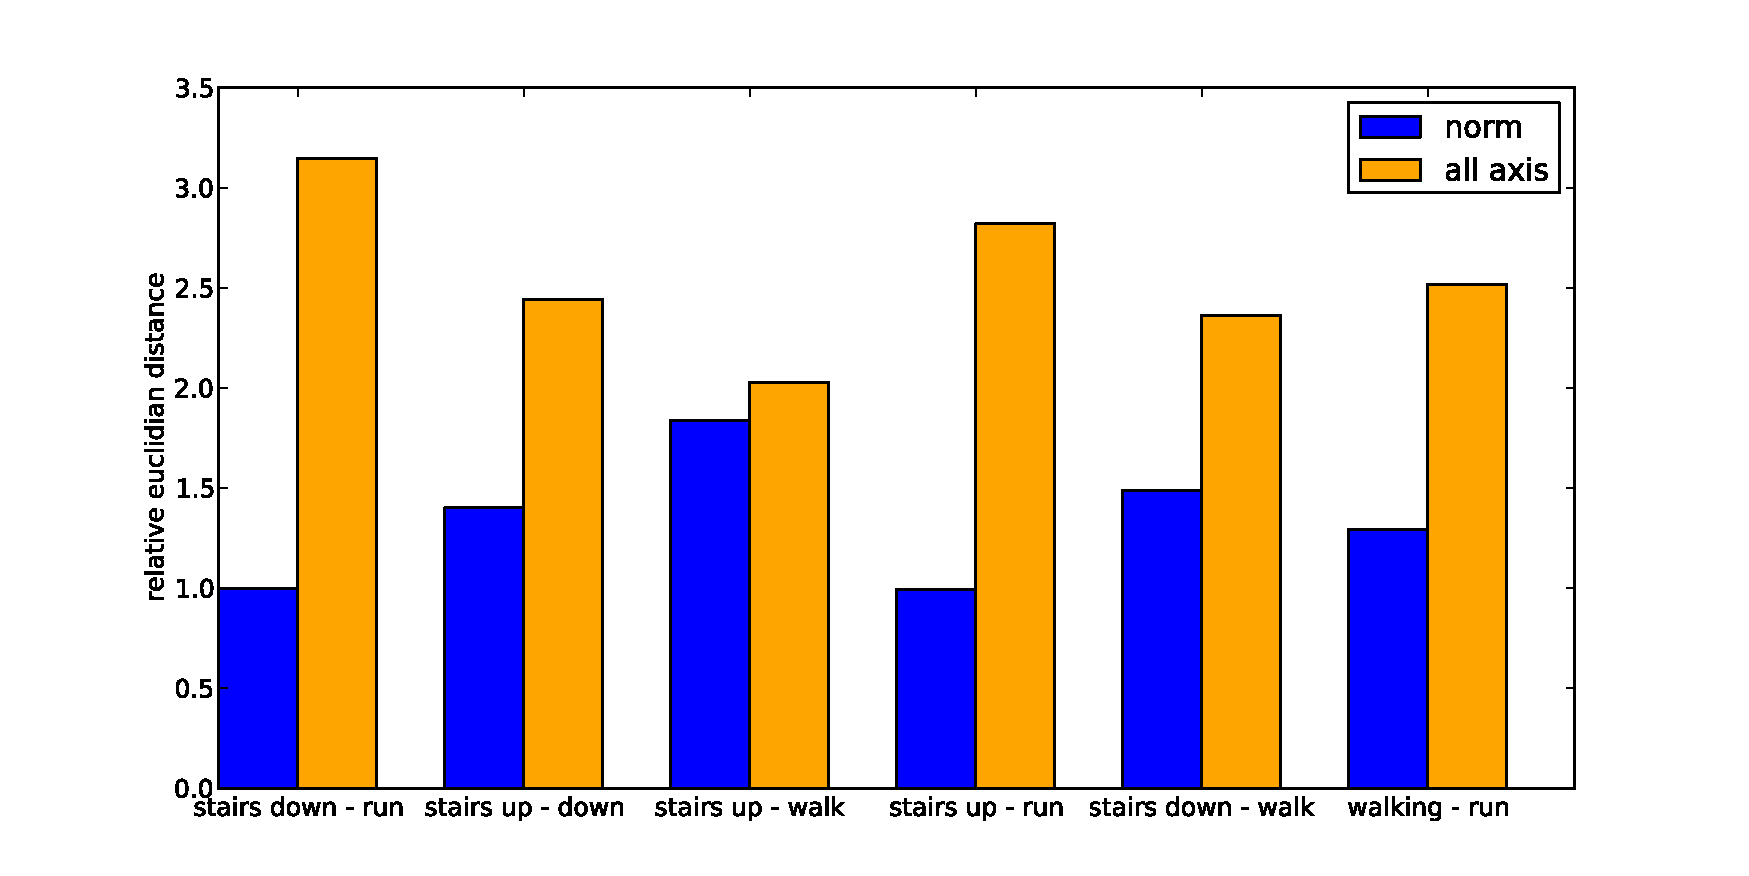
\includegraphics[height=2.5in]{orientAccel}
	\end{center}
\caption[Loss of orientation information]{ Illustrating the information loss for motion sensor based activity recognition, if device orientation information is disregarded. See the text for
 detail.} \label{fig:orientation} \end{figure}

In most cases motion sensors enabled devices are equipped with 3-axis
sensors. As a consequence the norm of the signal can be used as a
simple, orientation invariant signal. Thus, the interesting question
is not as much "what influence rotation has on the motion signals?",
but "how much information is lost when discarding orientation
sensitive features?" . 

The information loss in a very simple context
example is illustrated in Figure~\ref{fig:orientation}.
To show how orientation can provide better features, we consider
a standard mode of locomotion recognition problem: distinguishing
walking upstairs, downstairs, running and level walking. 
In Figure~\ref{fig:orientation} we use euclidean distance as measure of similarity 
to compare how well those classes are separated by (1) the norm and (2) orientation sensitive signals from the 3
individual axis of an accelerometer signal. Even
for such simple classes (which can actually be recognized reasonably
well using the norm), orientation sensitive feature contain
significantly more information.

As dedicated application feature, device orientation is particularly
relevant for systems that contain a magnetic field sensor (as is
increasingly the case with modern smart phones). Knowing the
orientation of the magnetic sensor axis with respect to the user's
body means that the sensor can be used to determine the direction in
which the user is facing. 
\begin{figure}[t]
  \begin{center}
  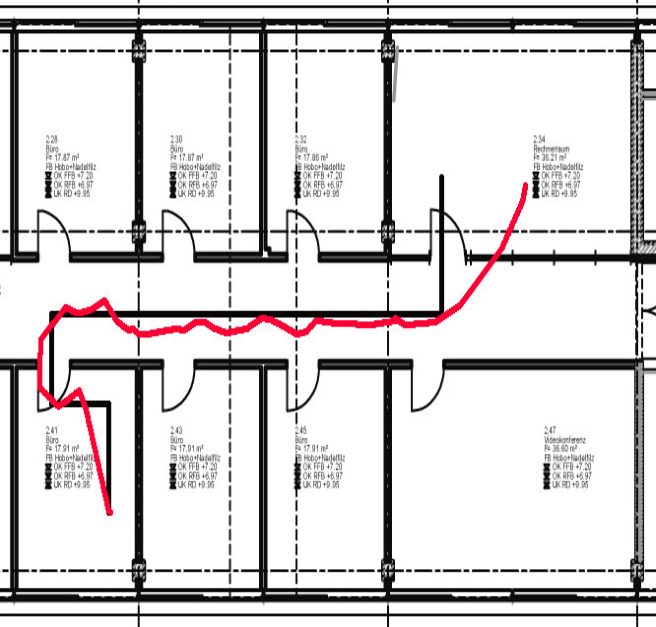
\includegraphics[height=1.5in]{deadreckoning}
	\end{center}
\caption{Dead-reckoning trace from accelerometer and magnetic field sensor of iphone 3gs, using the accelerometer to count steps
and the magnetic field sensor for direction (the black straight lines are the ground-truth, the other path the estimated trace).}
\label{fig:footsteps} \end{figure}
The direction the user is facing can indicate the focus of attention and 
provide information on social interactions, the use of household
devices, or interest in specific objects (e.g. a specific shelve in a
store indicating interest in certain products). Combined with step
detection, a magnetic field sensor placed on the body in a known
orientation can also be used as a simple yet effective means of indoor
navigation. This is illustrated in Figure Figure~\ref{fig:footsteps}.
It shows a walking path estimation using the accelerometer of an
iphone 3gs for step counting and the built-in magnetic sensor to
obtain the orientation. The only additional processing done to the
graph is to apply a Kalman Filter to the orientation data. This method 
is fundamentally different (and much simpler) from the
standard indoor navigation approach where the information from a 3
axis accelerometer, gyro and magnetic field sensor is integrated over
time and the device orientation is not required.

\section{Detecting Device Orientation}
\label{sec:orientationdetection}
When estimating the orientation of a device with respect to the user's
body, two distinct sub-problems must be distinguished: vertical
orientation (angle with respect to the gravity vector) and the
orientation in the horizontal plane.

\subsection{Orientation in the Vertical Plane}
As has been first proposed by Mizel~\cite{Mizell:2005p3885}, vertical
orientation can be easily estimated when the object experiences no
change in motion speed. In this case the only acceleration registered
by the sensor is the earth gravity (9.81 $m/s^2$) and the direction of
the measured acceleration vector defines the vertical plane. To
identify signal segments with the above characteristics the norm of
the measured acceleration vector is used together with its
variance. When variance of all axis tends towards 0 and the norm
vector approaches 9.81 $m/s^2$, the signal is very likely to be
dominated by the vertical orientation component \footnote{In theory
 this needs not be the case since the object could for example be
free falling (no gravity component) while experiencing a constant 9.81
$m/s^2$ along an arbitrary direction.}.
 
 \subsection{Horizontal Orientation}

We present a method to infer the orientation of a mobile device
carried in a pocket from the acceleration signal acquired when the
user is walking. Whereas previous work has shown how to determine the
orientation in the vertical plane (angle towards earth gravity), we
demonstrate how to compute the orientation within the horizontal
plane.

%A major issue that has to be considered is the fact that users carry
%such devices in a variety of ways. In general neither the location
%(pocket, belt, bag) nor the orientation of the device can be assumed
%to be known. In previous chapters, we demonstrated how to detect where
%on the body the device is located by analyzing the accelerometer
%signal during various activities~\cite{Kunze:2007p86}. We have also
%shown how to deal with sensor displacement~\cite{Kunze:2008p6845}. 
In the following, we show how to infer the orientation of the device with
respect to the user's body. We extend existing work by
~\cite{Mizell:2005p3885} that has shown how the orientation in the
vertical plane (angle towards gravity) can be computed by additionally
inferring the orientation in the horizontal plane. Our method is based
on the observation that while walking, the most variations in the
horizontal plane of the acceleration signal will be parallel to the
direction of motion. To distinguish between front and back we look at
the integral of the signal over time.

We focus on the trouser pocket, as it is by far the most likely
placement for peoples mobile phones (see~\cite{Ichikawa:2005p6295}).
This work is partially inspired by Blanke
et. al.~\cite{Blanke:2008p6128}. We base the approach on three
assumptions:
\begin{itemize}
\item The user walks facing forward.
\item The device is placed in a trousers pocket. Our approach should
 also yield similar results on the person's torso or similar on-body
 placements. However, we did not test them in this thesis.
\item We apply our approach on a walking segment in which 
the user walked fairly straight.
\end{itemize}
As already described by Mizel~\cite{Mizell:2005p3885}, one can
estimate the gravity vector component of a 3-axis accelerometer. We
use a slight variation of this method to get the acceleration axis
parallel to the persons torso: We apply a sliding window over over all
3 axes. If the variance of all axes is close to 0 and the magnitude
approaches 9.81 $m/s^2$, the signal is very likely to be dominated by
the vertical orientation component.
\begin{figure}[!t]
\centering
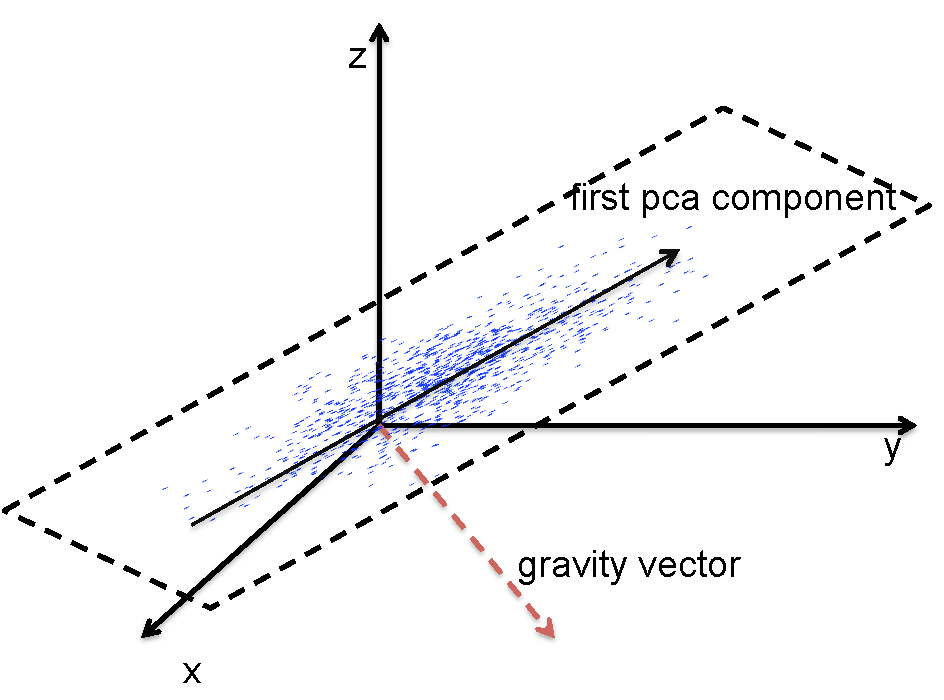
\includegraphics[width=2in]{pca}
\caption[Accelerometer coordinate system]{Accelerometer coordinate system in relation
to the gravity vector (vertical component) and the walking
direction infered using pca.}
\label{fig_pca}
\end{figure}

Using this heuristic, we infer the vertical component.
Now we project the accelerometer signal in the plane
perpendicular to the vertical gravity vector (=horizontal plane). 
We apply principle component analysis on the projected
data points (see Figure~\ref{fig_pca}) to get the direction where the
acceleration variations is greatest.  This is the axis that is
parallel to the walking direction. Assuming that the user is walking
forward, integration over the component will allows us to determine
which way is front (leads to positive integral) and which is back
(see Figure~\ref{fig_integral}). 


\section{Experimental Evaluation}

We test the approach described above with the following setup.
We use a MTx motion sensor (equipped with 3-axis accelerometer, gyro
and magnetic field) with a custom bluetooth sender placed in a mobile
phone casing as data source for our algorithm. As reference we use a
GPS device. We stream all data to a Nokia N810 running the context
recognition network toolbox\footnote{http://crnt.sf.net} for recording
and labeling.

In the MTx box, the magnetic field sensor axes are
oriented in parallel to the acceleration sensor axes. Therefore,
if our algorithm can infer the orientation of the acceleration axis
with respect to the user's body we automatically have the orientation
of the magnetic field sensor with respect to the body. This is
equivalent to knowing which way (in terms of longitude and latitude)
the user is facing. If the user is walking forward this direction is
also the user's heading. By comparing the heading computed this way
with the heading provided by GPS we can verify the accuracy of our
method for determining the horizontal orientation of the sensor.

Two test subjects walked a straight path outside (around 30 meters)
with the MTx sensor in the right trouser pocket and the GPS in hand.
We repeat this experimental setup 8 times per person changing the
sensor orientation each time. We pick only 8, comparing the device
to a mobile phone, users will most likely not place the device with
the thin side facing towards the body. So we place the phone casing
with the sensor in the right trousers pocket facing front rotating it
90 degrees further for each experimental trial (the same procedure with
the backside facing front), leaving us with 8 distinct orientations.

\begin{figure}[!t]
\centering 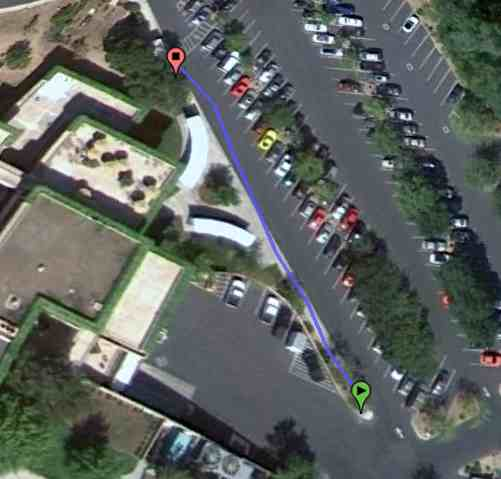
\includegraphics[height=2in]{trace}
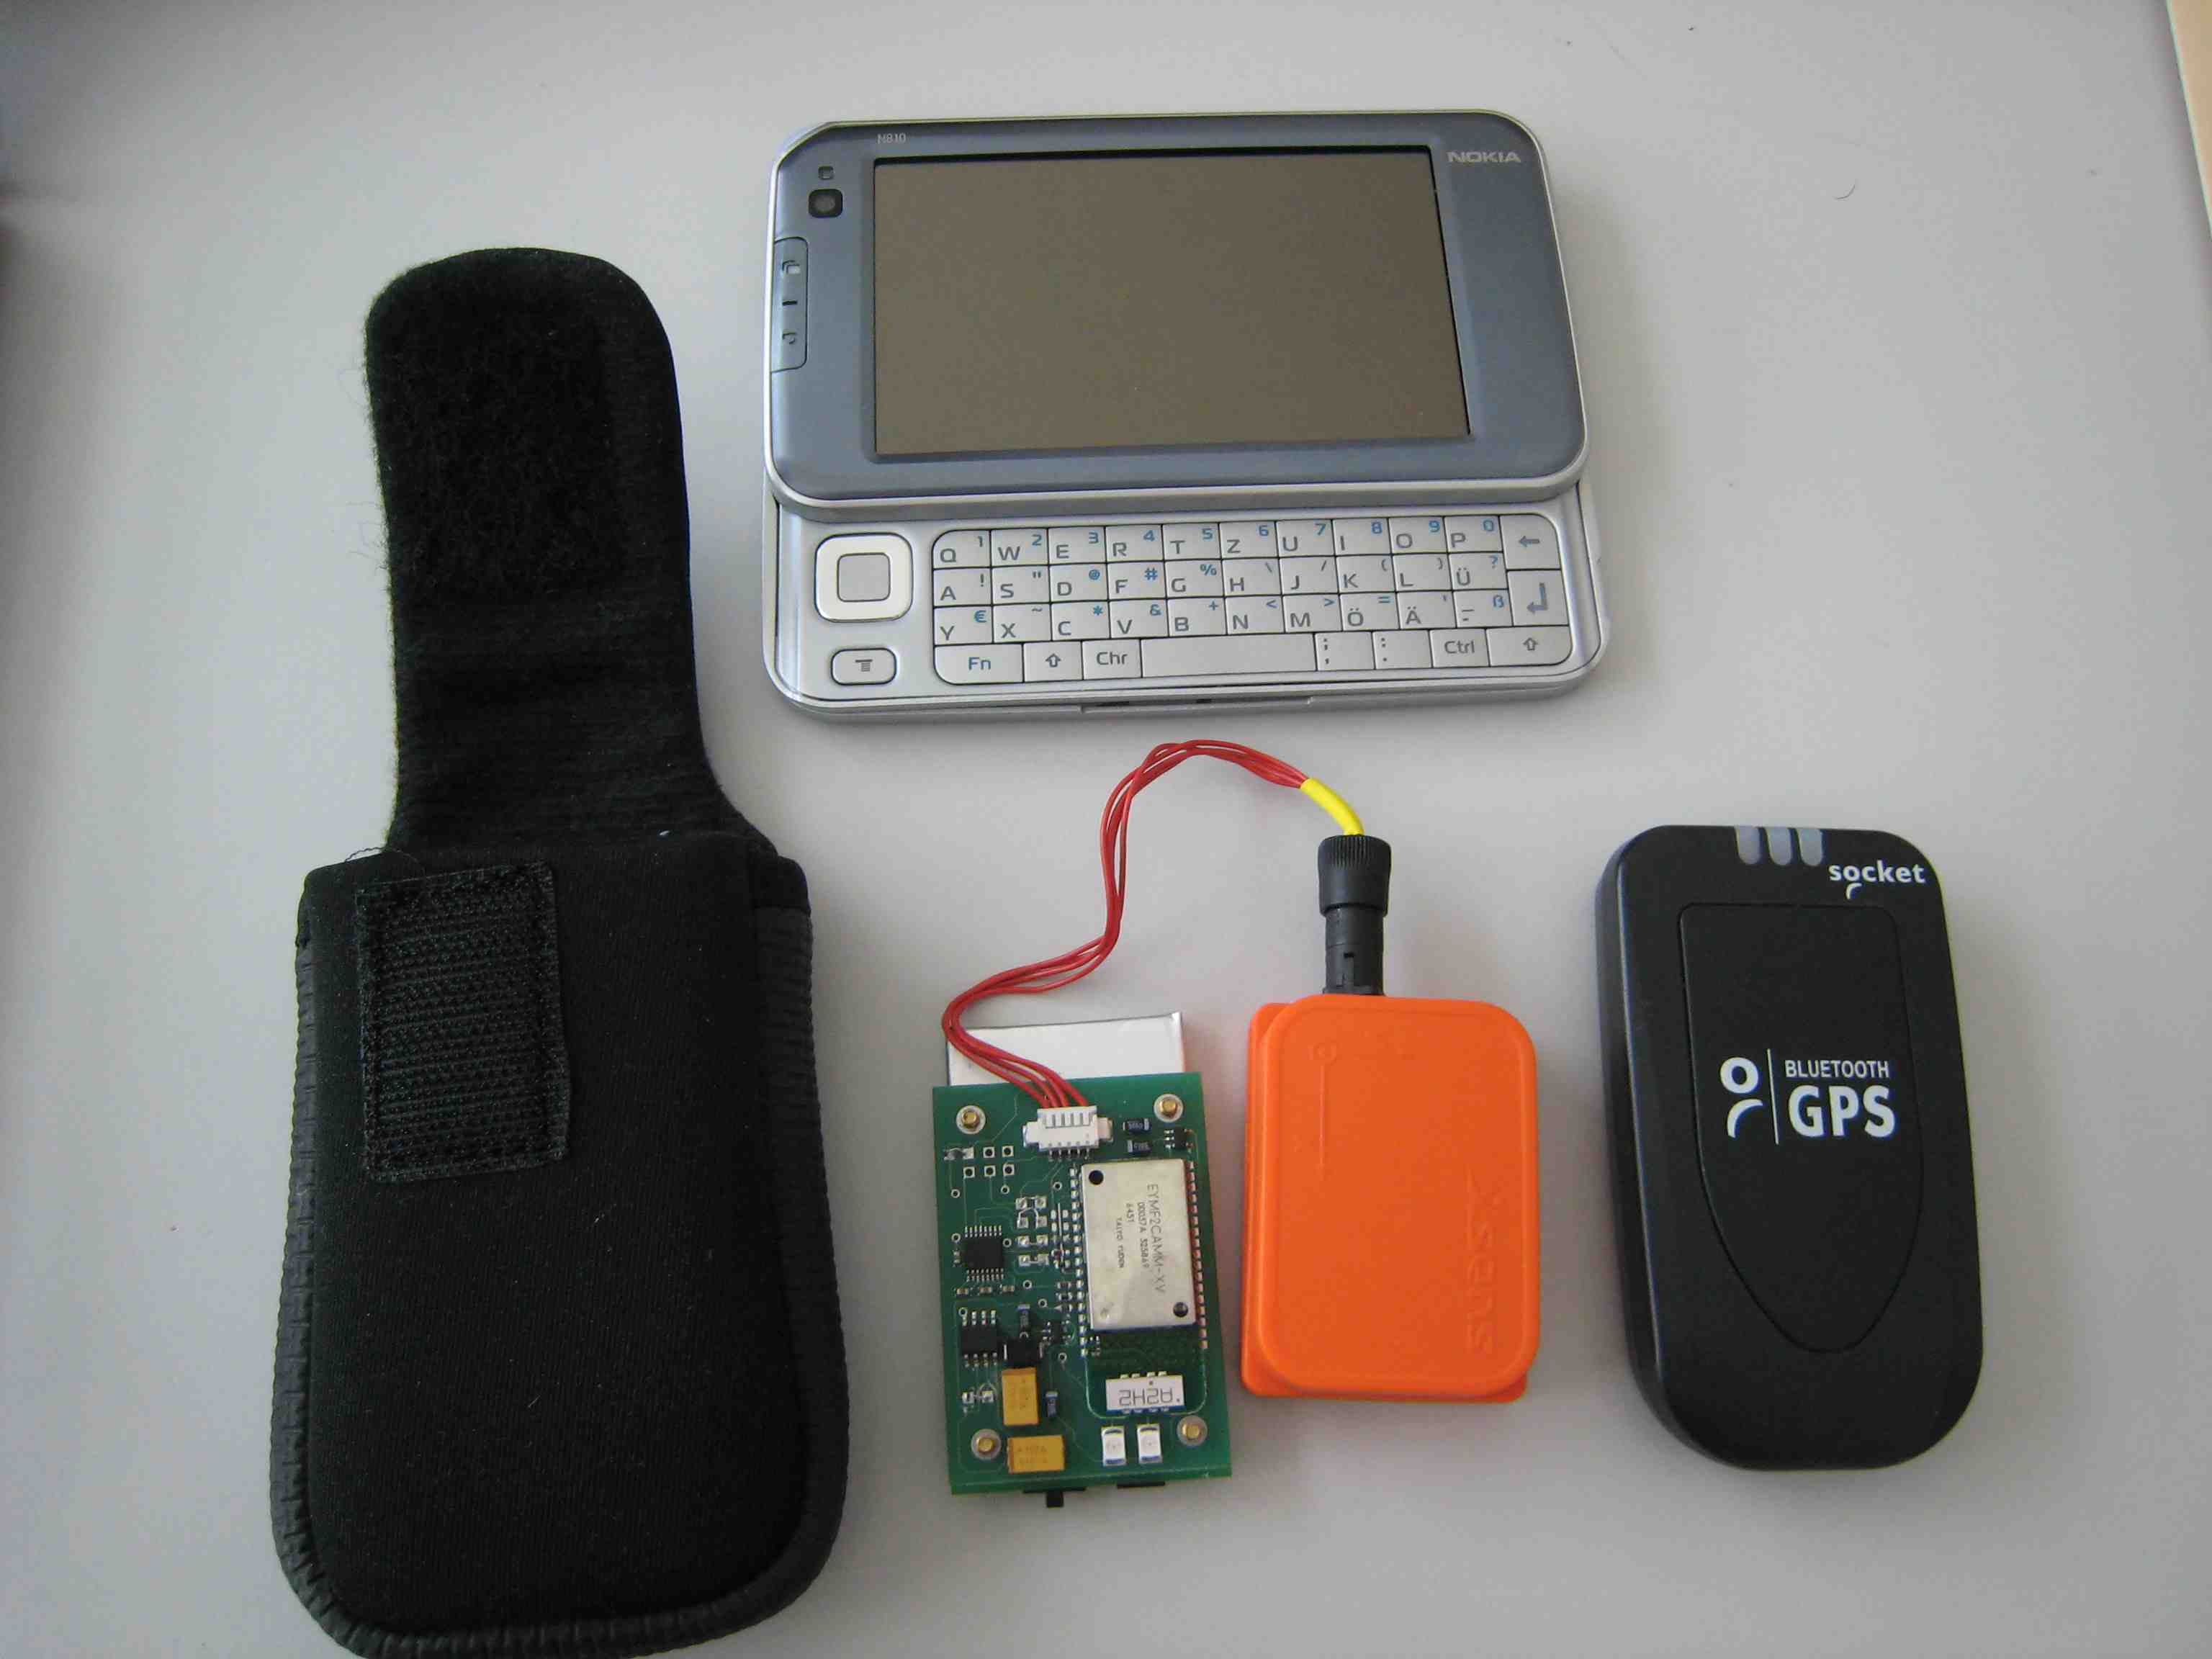
\includegraphics[width=2in]{devices.jpg}
	
\caption[Experimental setup]{Sample trace and equipment used for the experimental setup: a
 mobile phone box, MTx motion sensor with bluetooth adapter, nokia
 810 and a gps device.}
\label{devices}
\end{figure}

\begin{figure}[t]
\centering  
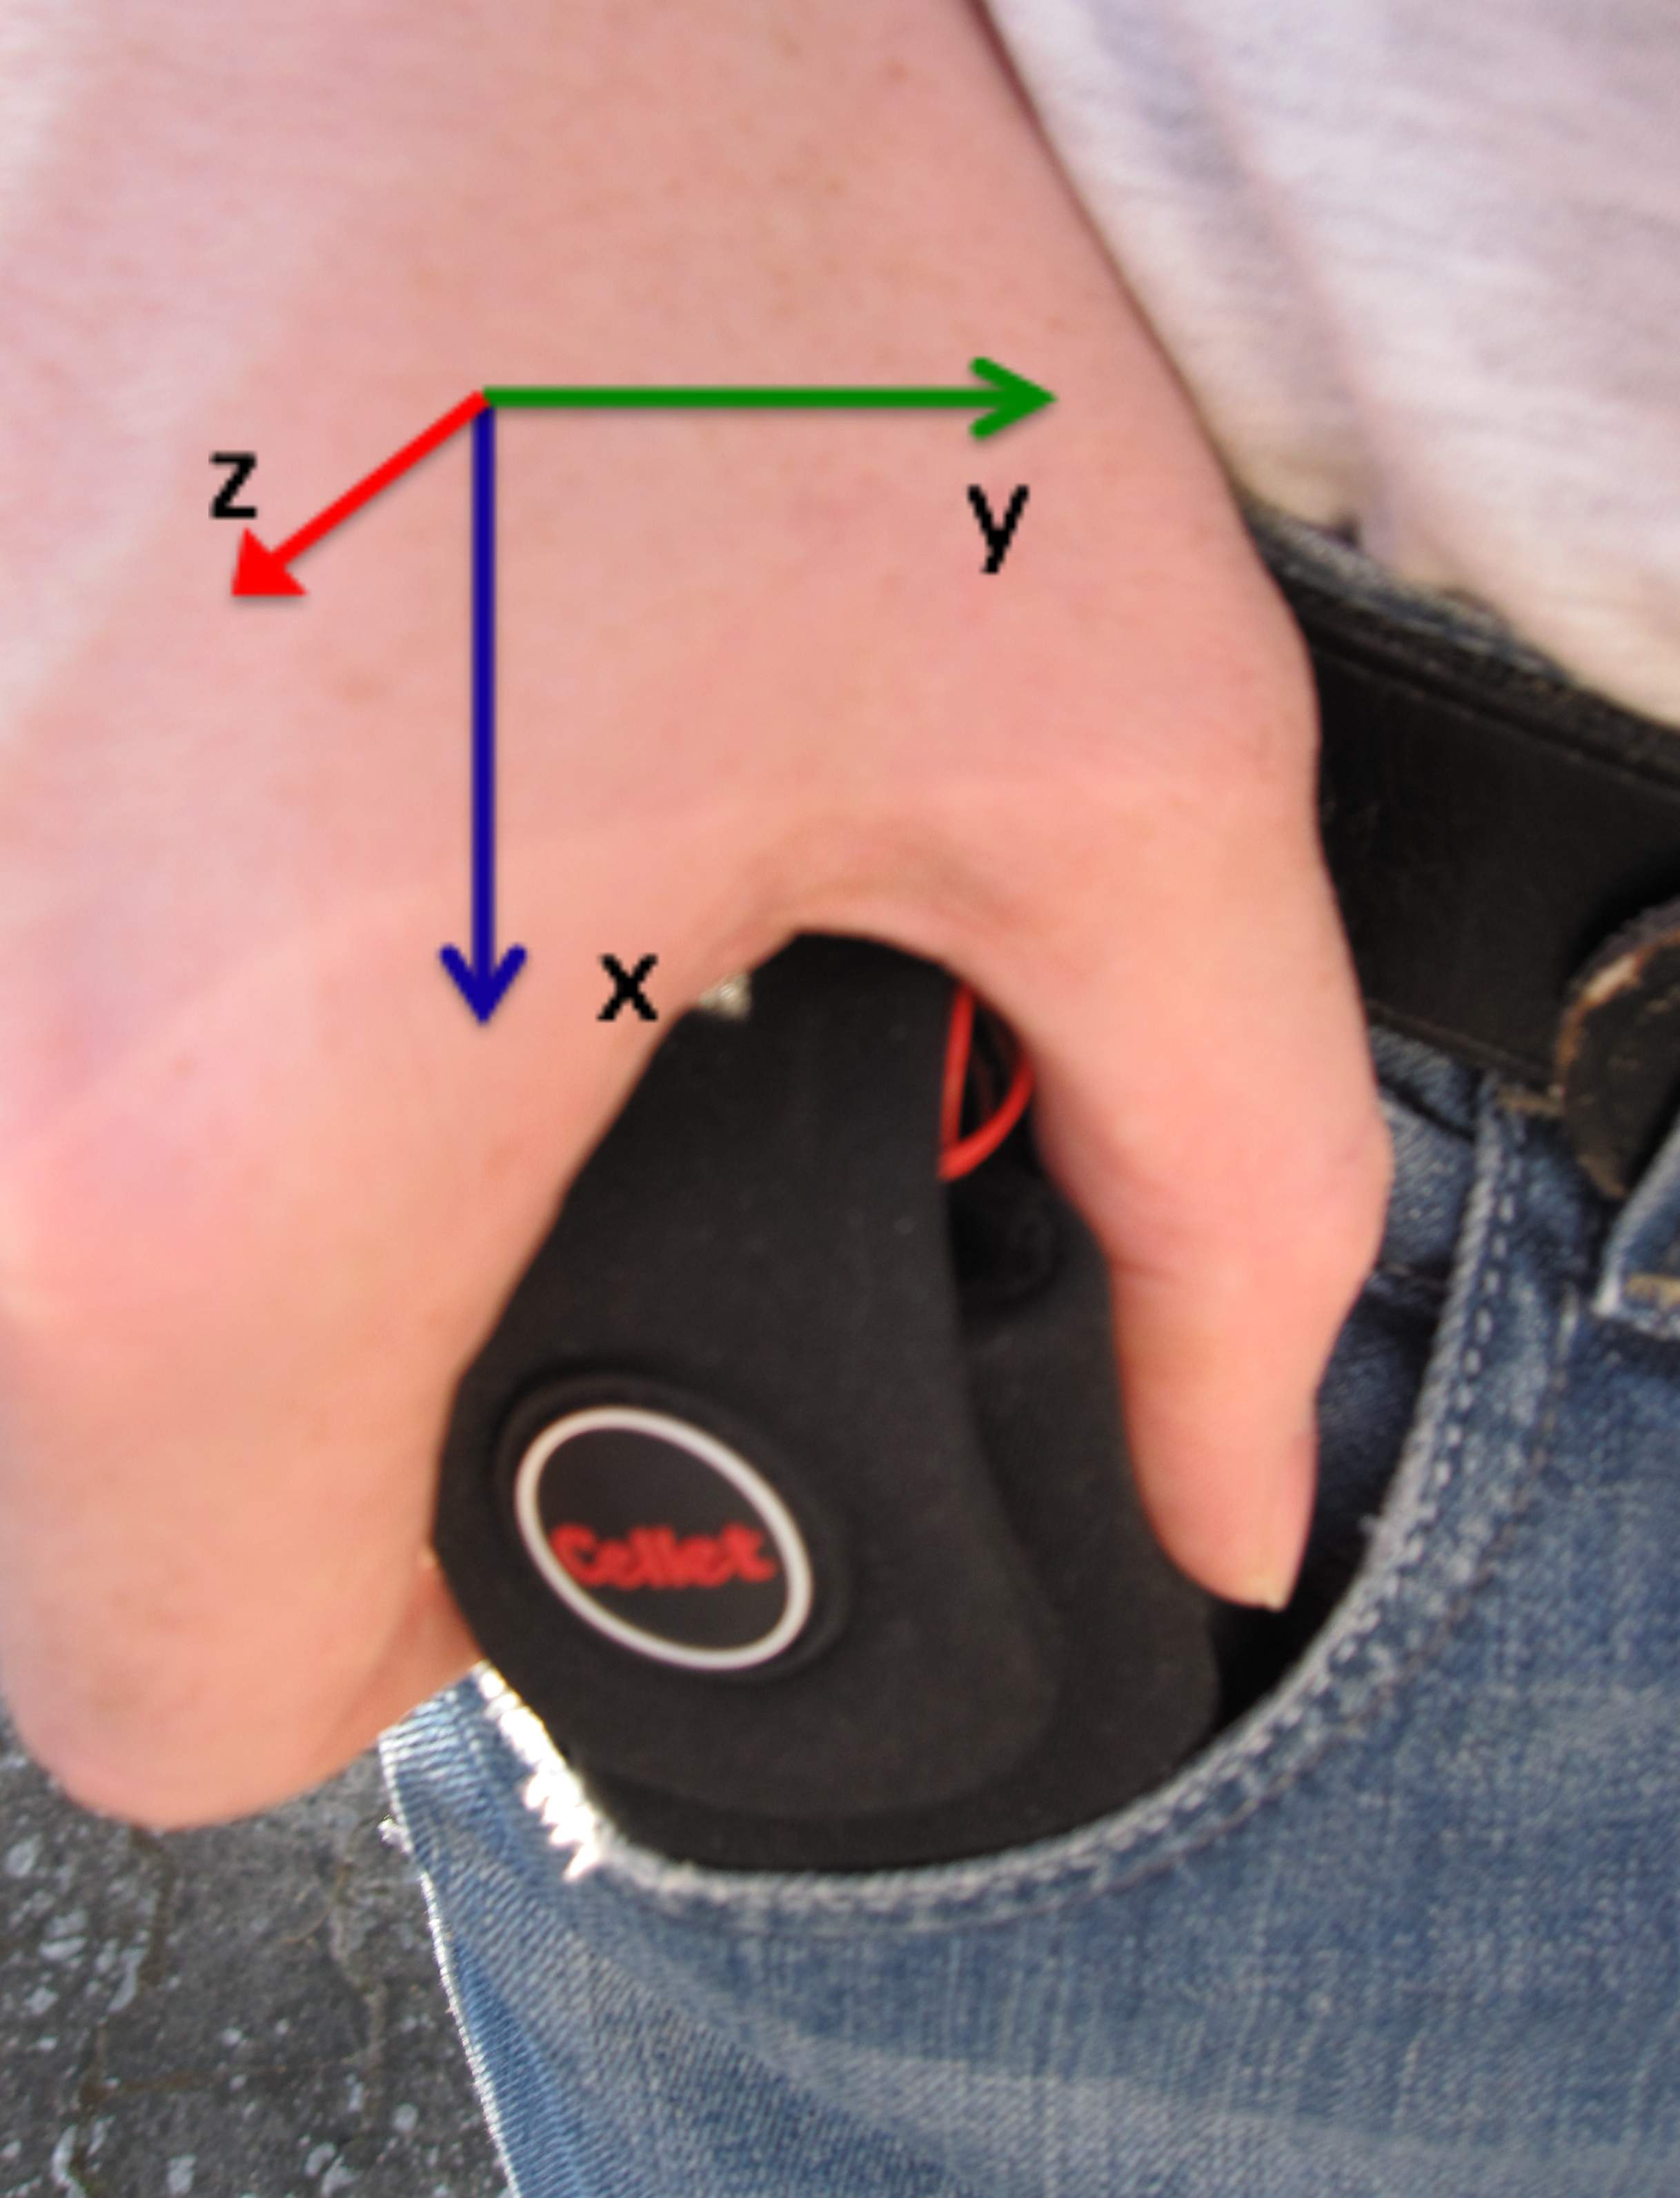
\includegraphics[scale=0.075]{sdown.jpg}
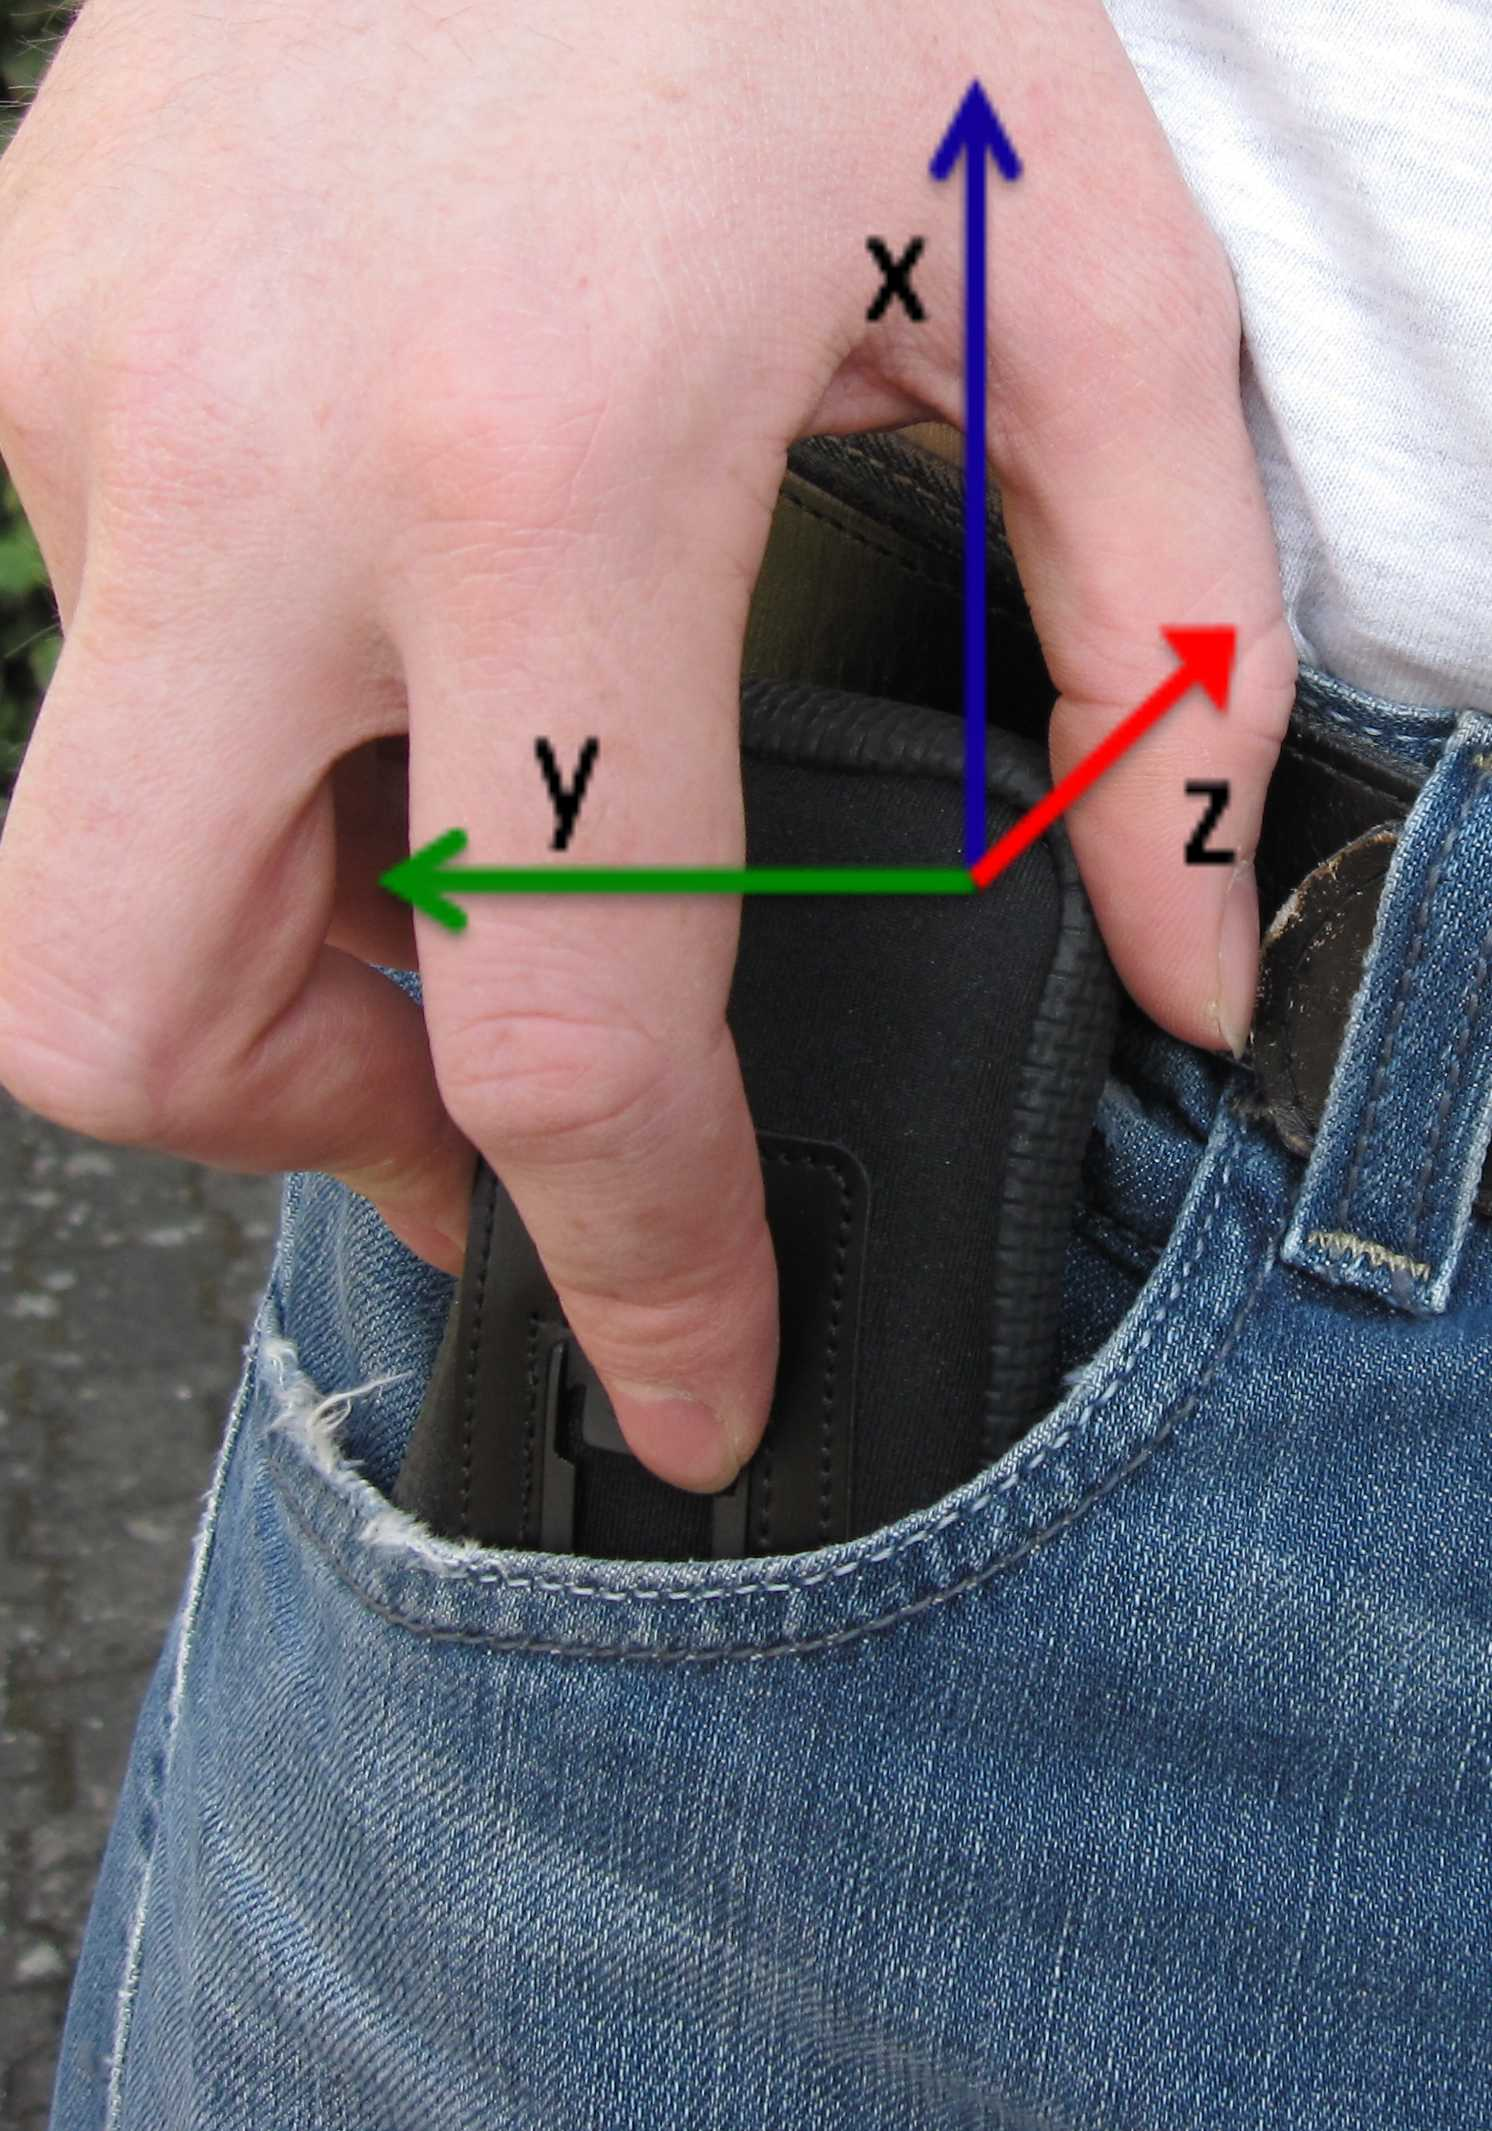
\includegraphics[scale=0.112]{sback.jpg}
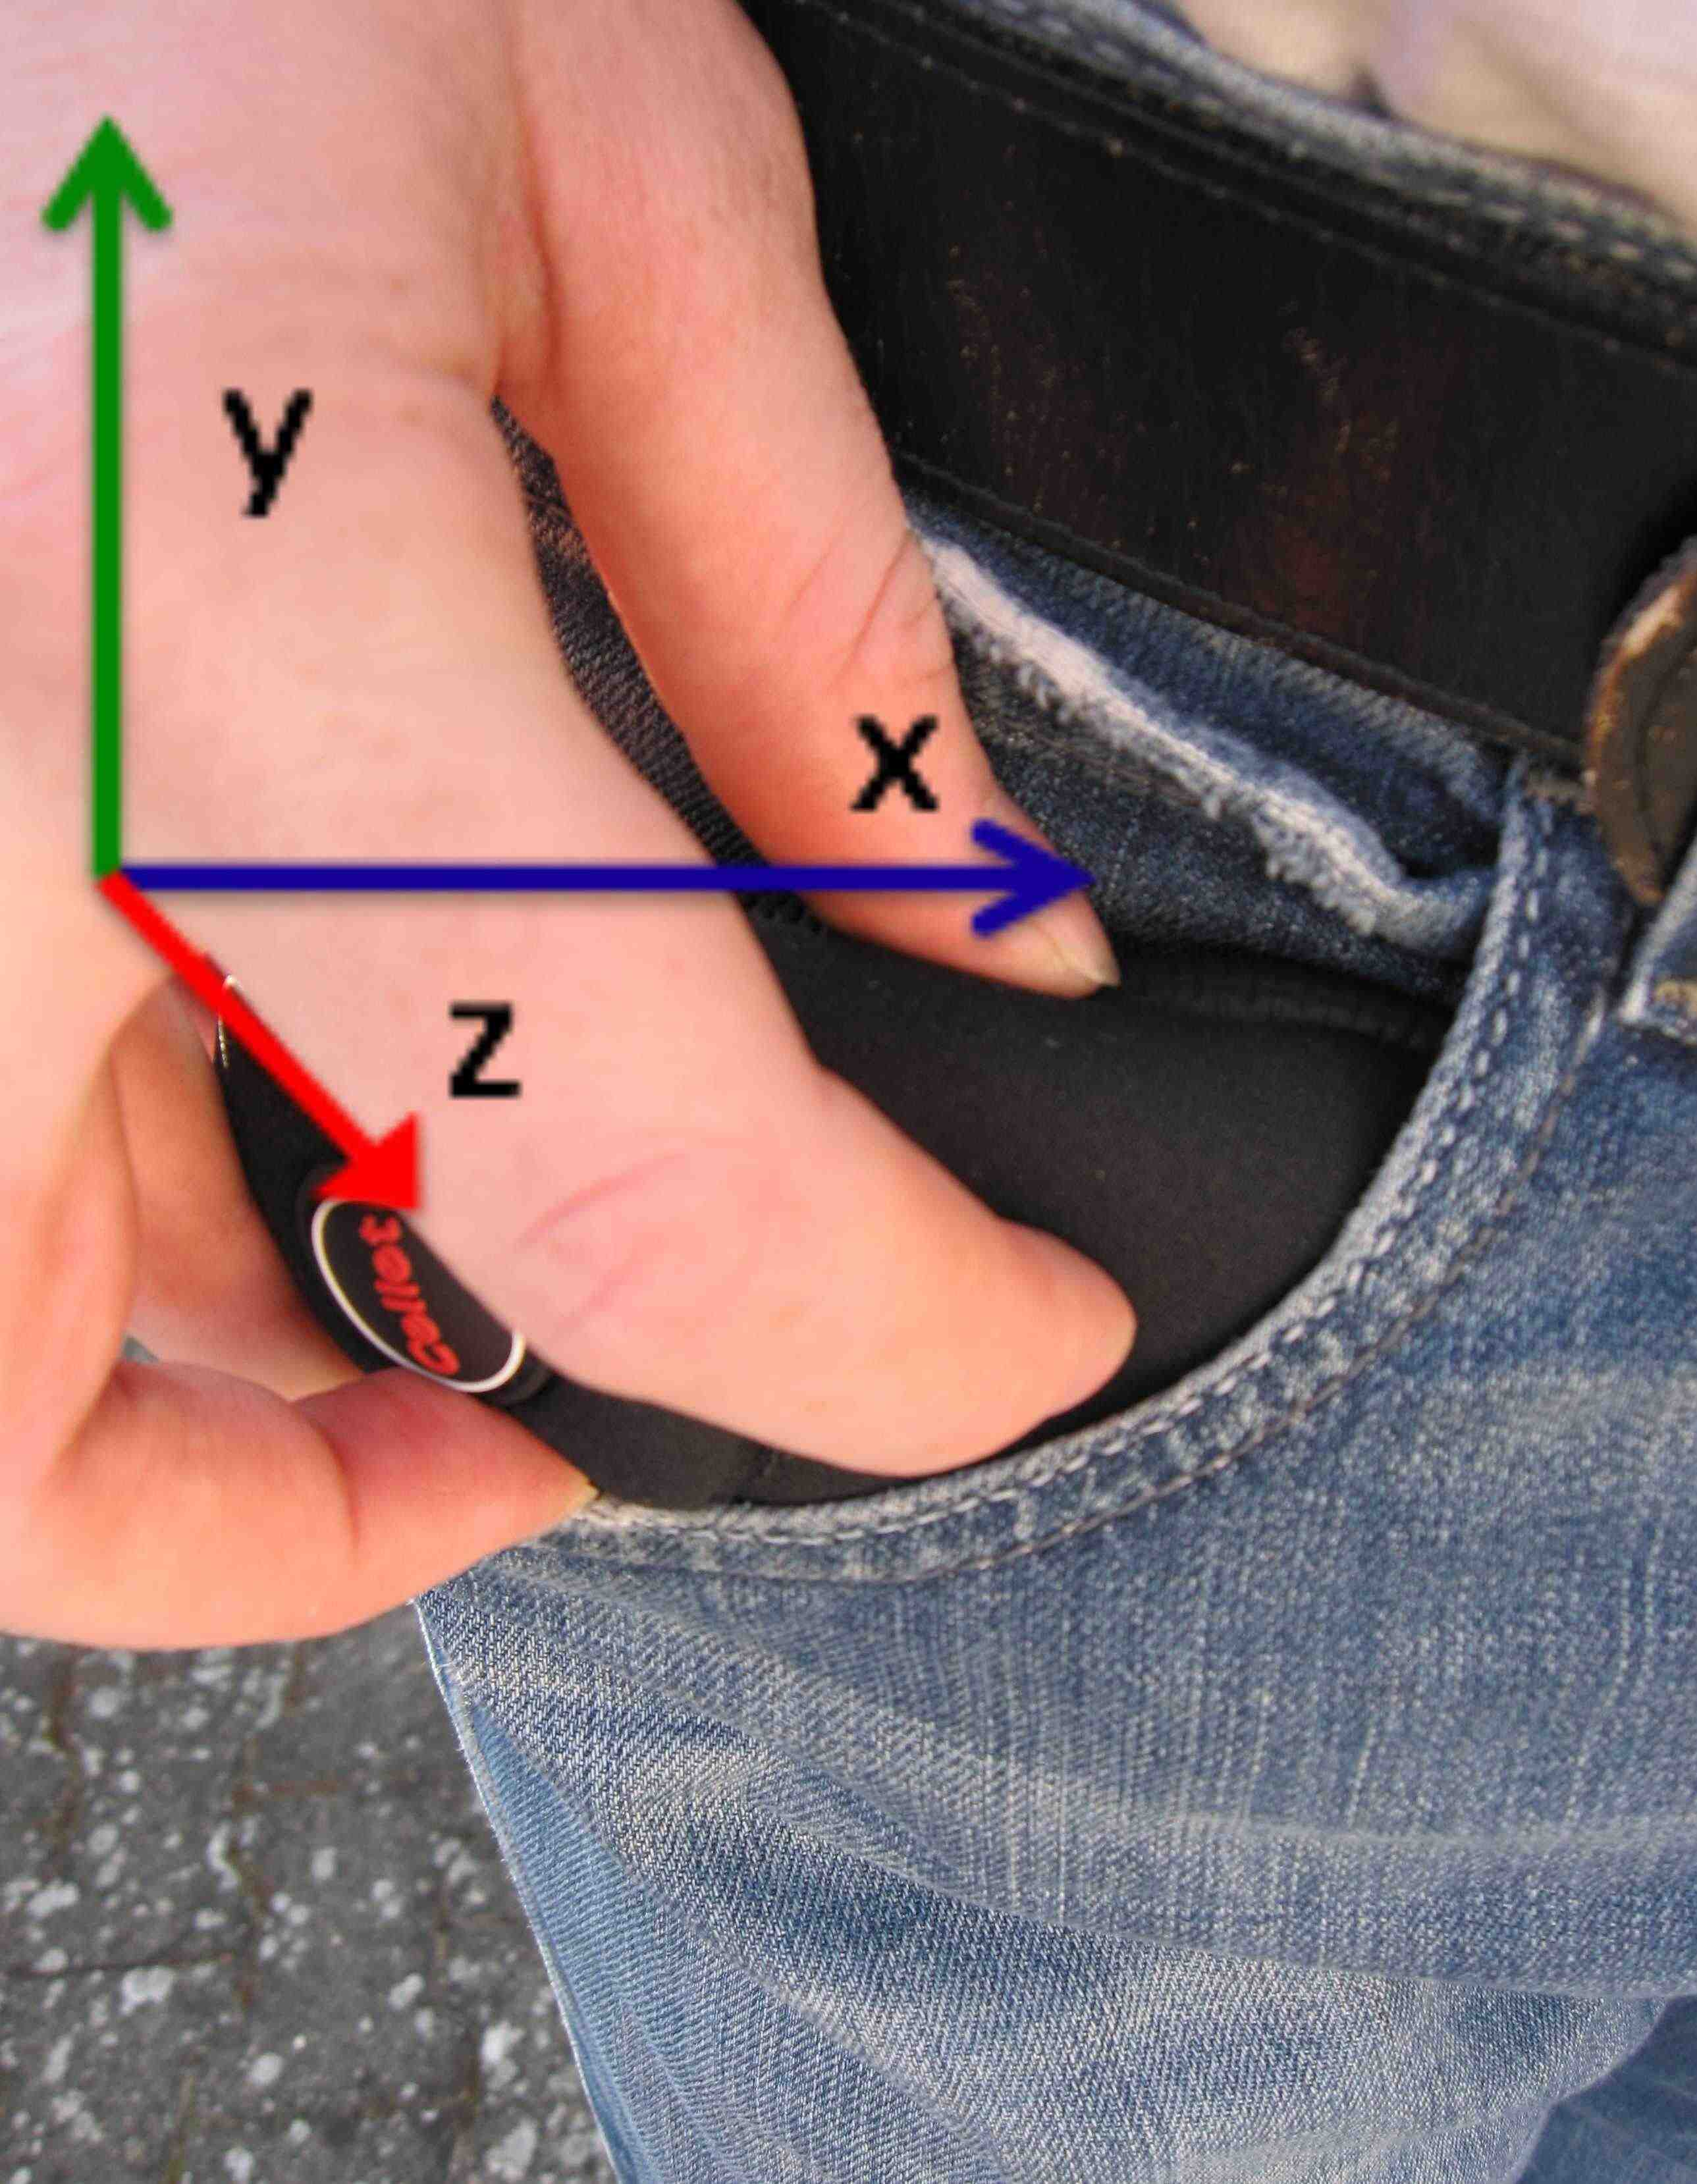
\includegraphics[scale=0.0724]{sside.jpg}
\caption[Device orientations]{The Mtx motion sensor in the phone casing placed in the pocket 
depicted with the different axis orientations.}
\label{fig:devices}
\end{figure}

\begin{figure}[!t]
\centering
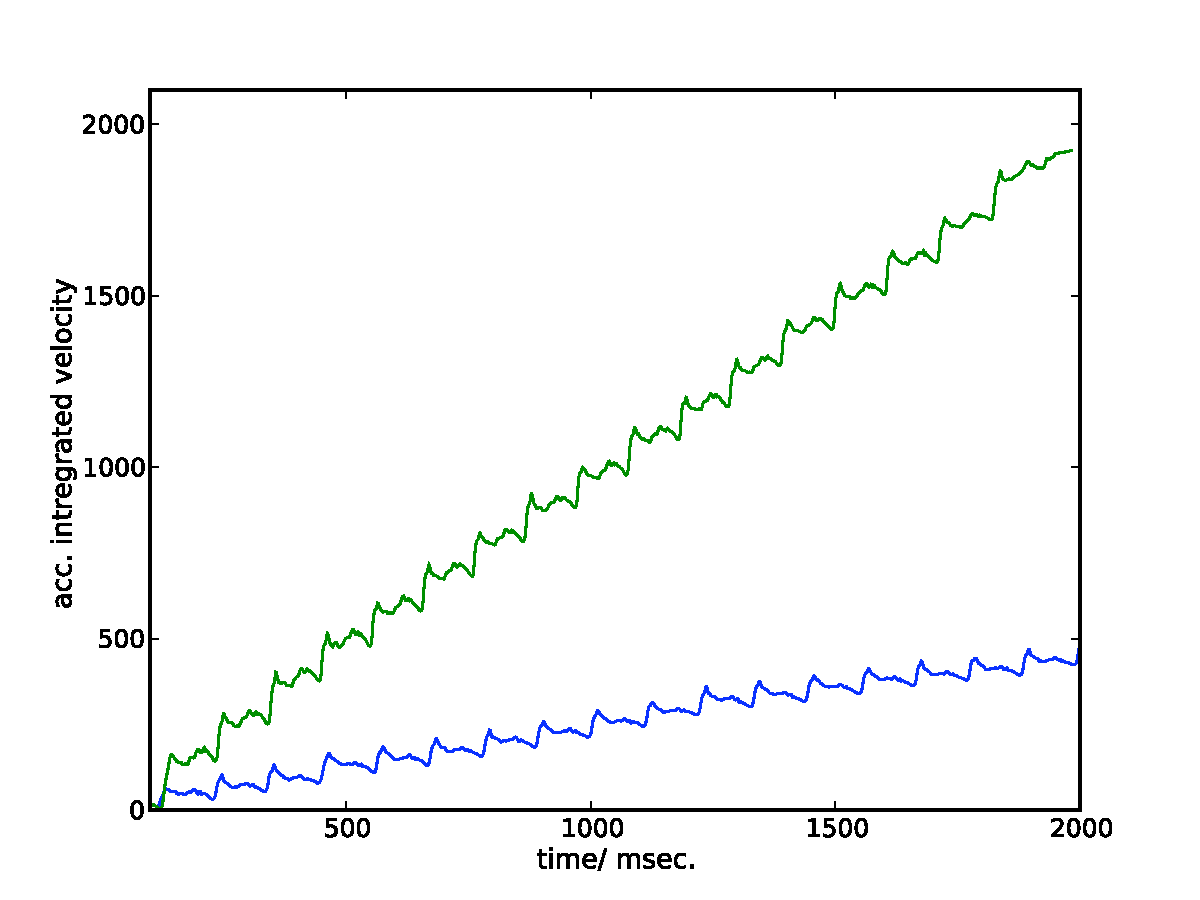
\includegraphics[width=3in]{integral}

\caption[Integrated velocity]{The accumulated integrated velocity of the first pca component direction
for 2 trials with different sensor orientations, one in which the test subject 
was walking slowly (blue) and fast (green).}
\label{fig_integral}
\end{figure}
Three of the 8 orientations are shown in Figure~\ref{fig:devices}.
Using the approach presented above, we can reliably detect the side of the sensor
facing in walking direction for all of the 16 experimental trials. Figure~\ref{fig_integral}
shows an incremental integration over the principal component acceleration axis for a person
walking slow (blue graph) and walking fast (green graph) with different sensor orientations.

\begin{figure}[!t]
\centering
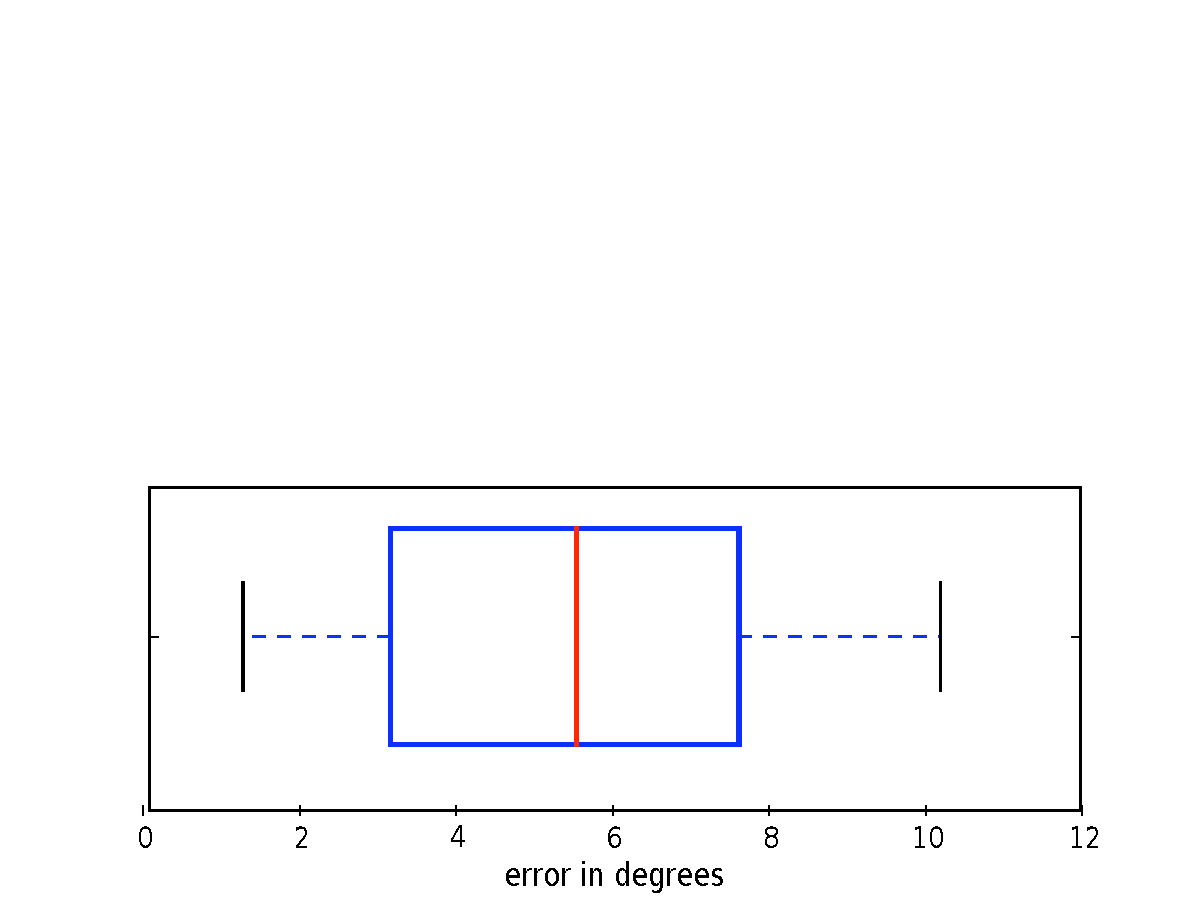
\includegraphics[width=2.5in]{error}

\caption[Error between accelerometer and gps]{The errors between the accelerometer and gps based approaches, mean at around 5 degrees 
with a standard deviation of 2.5 degrees.}
\label{box_plot}
\end{figure}

To validate our method we compare its output with GPS heading
information when walking in a straight line. On a total of 16
different orientations and traces we have a mean difference of 5
degrees with 2.5 degrees standard deviation, as depicted in
Figure~\ref{box_plot}. .

\section{Conclusion}
During most longterm sensor deployments orientation shifts are to be expected. Especially Context sensing using smart phones benefits
from device orientation inference, as smart phones are often loosely placed in a pocket or bag~\cite{Ichikawa:2005p6295}.
As seen from the impact analysis in Section~\ref{orient:impact}, shifts in orientation do not only affect motion sensors. Large changes in device orientation with respect to the user's body can influence the signal quality of sound and radio signals, if the microphone/antenna has strong directional characteristics. 
Therefore, we believe that the work presented in this chapter constitutes an important contribution to dealing with sensor placement effects in activity recognition.

With respect to motion sensors, the vector norm can be used as an example of an orientation-invariant feature. However, ignoring orientation means losing information. Thus, we showed how to derive both vertical and horizontal orientation using only an
accelerometer signal. Our proposed method to infer orientation is comparable to using the
Euler Angles and GPS. However, it only uses an accelerometer and is not limited to being outside (gps) or susceptible to metal (magnetic compass).
Of course, the method introduced has its limitations. Most importantly, we assume some rest periods in which the vertical plane to gravity can be determined.
Also, our experiment shows the approach only working, if the user walks on a straight line. Though both limitations are not as severe as they might sound.
Rest periods should happen quite often, if the user carries the device during a regular day. Only a fraction of a second is enough to determine the 
gravitational pull. In addition, the proposed method should also work on "not straight walking". If further experiments show that this is not the case, 
it should be feasible to detect straight walking (utilizing a gyroscope or magnetic compass, see~\cite{sekine2000}). Then the method would work again with the cost of an additional sensor. 


Some immediate future work ideas include to try the method on curved walking segments and to extend the approach to continuous device orientation 
tracking. Our method can be used to give an initial orientation estimate and periodic updates, in between one can utilize the relative device orientation libraries of popular smartphones (Android and iPhone) or a method based on a similar approach Foerster et. al. introduced for displacement (see~\cite{Forster1}).

Inferring the device orientation concludes our discussion on placement variations in sensor signals.


\bibliographystyle{abbrv} \bibliography{Orientation}
